\section{Assessment of Pain}
Pain is described as a complex and subjective experience that poses a number of measurement challenges due to its subjective nature. Nevertheless, pain measurements are necessary for pain studies as well as the evaluation of methods to control pain.~\cite{Jensen2001} %There is no valid and reliable method of objectively quantifying pain at the moment. 
Despite the challenges that pain measurement present, several tools and approaches can be employed in order to collect useful pain estimates.~\cite{Younger2010} The aim of pain assessment is to diagnose the cause, understand the impact, identify appropriate pain relief strategies and evaluate their effectiveness~\cite{Briggs2010}.

%There are different dimensions of pain experience that can be assessed: intensity, affect, quality and location. Pain intensity defines how much the pain hurts. %, where pain affect is more complex. 
%Pain affect refers the degree of emotional arousal or changes in action due to the sensory experience of pain. Whereas pain quality concerns certain physical perceptions, which are associated with the description of pain, such as pins and needles, prickling or burning. \cite{Jensen2001}

The intensity of pain can be assessed using unidimensional or multidimentional scales ~\cite{Jensen2001}.
 % Changes in pain intensity should only be compared individually and not between subjects, as pain is a subjective experience.
Chronic pain is too complex to assess with unidimensional scales, as the pain affect the patients' functions, quality of life, emotional state, vocational status, social life and well-being, wherefore multidimensional scales are used~\cite{Ebert2010}. 


\subsection{Unidimensional scales}
One used unidimensional scale is the Verbal Rating Scale (VRS), which consists of a list of adjectives describing different levels of pain intensity, as illustrated in \figref{fig:VRS}. This type of scale is easy to administer, score and apprehend. However, it has several statistical disadvantages and criticism raised due to the fact that it assumes equal intervals between the adjectives.~\cite{Jensen2001} For this particular reason along with others, it is only used when the patient's conditions require it~\cite{Jensen1986}. 

\begin{figure}[H]
	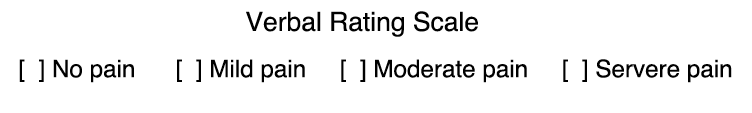
\includegraphics[width=0.5\textwidth]{figures/VRS.png} 
	\caption{Verbal Rating Scale (VRS). Modified~\cite{Jensen2001}.}
	\label{fig:VRS}  
\end{figure}   

Another possibility of unidimensional scales is a Visual Analogue Scale (VAS). VAS consists of a 10 cm line, as shown in \figref{fig:VAS}. The ends of this line are labeled as the extremes of pain. The scale is scored by measuring the distance from 'no pain' to the patient's mark. This fact makes the VAS more sensitive to changes in pain intensity. However, one of the drawbacks is its evaluation time is higher than for other methods.~\cite{Jensen2001} 

\begin{figure}[H]
	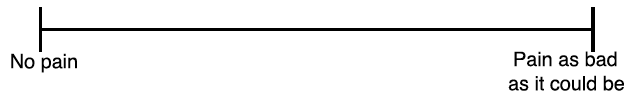
\includegraphics[width=0.5\textwidth]{figures/VAS.png} 
	\caption{Visual analogue scale (VAS). Modified~\cite{Jensen2001}.}
	\label{fig:VAS}  
\end{figure}   

Another method is the Numerical Rating Scale (NRS), which is illustrated in \figref{fig:NRS}. It is the most used by clinicians, due to the usefulness of administration and scoring \cite{Fillingim2016}. NRS consists of a numerical scale from 0 to 10, describing 0 as 'no pain' and  10 as 'higest level of pain'. The advantage of NRS is that it does not require patients' mobility because the response is given verbally. NRS is a valid method and demonstrates positive and significant correlations with other measurements of pain intensity. \cite{Jensen2001} 

\begin{figure}[H]
	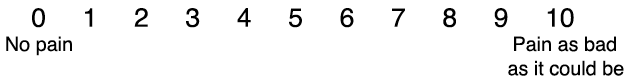
\includegraphics[width=0.5\textwidth]{figures/NRS.png} 
	\caption{Numerical Rating Scale (NRS). Modified~\cite{Jensen2001}.}
	\label{fig:NRS}  
\end{figure}   

Pictures or face scales can be used to illustrate facial expressions of different intensities of pain. The primary purpose of these scales is to offer individuals with written language or cognitive difficulties, an option to express pain intensity. There is evidence that the pictures or face scales are a valid method. \cite{Jensen2001} 

\subsection{Multidimensional scales}
Multidimensional scales are convenient in relentless pain conditions. There are several  multidimensional scales, whose purpose is to measure several dimensions of pain with different combinations of these dimensions. These scales offer a more detailed reflection of the patient's pain experience than unidimensional scales. \cite{Briggs2010} 

The most frequently used is McGill Pain Questionnaire (MPQ), which consists of 78 words and describes the pain in sensory, affective and evaluative terms. These terms are arranged in groups according to the quality and intensity of pain. A 6-point VRS is used to determine the intensity of the pain. One disadvantage of the MPQ is the length and complexity, wherefore a brief form of this questionnaire has been introduced. The short-form MPQ consists of 15 different descriptors in sensory and affected terms. Each descriptor is rated on a 4-point VRS scale.~\cite{Katz2001}

%Another scale, Brief Pain Inventory (BPI), was developed to assess cancer pain and has been proven as a useful instrument to asses different kinds of pain in several clinical settings. The BPI measures pain severity, pain quality and the disturbance in the patients' daily life. Two subscales score pain intensity and pain interference.~\cite{Katz2001} 

Pain drawing is often used for estimating the location of pain and involves a front and back drawing of the human body. Another used method is the checklist, which is a simple list of possible sites of pain.~\cite{Jensen2001} 


%\subsubsection{Physiological assessment}
%The most commend used for physiological assessment is Back Depression Inventory (BDI), which is used for patients with depression associated to their chronic pain. BDI consist of a questionnaire of 21 question related to the depression. The score of BDI indicated the if the depression is minor, moderate or server. The Spielberger-State-Trait Anxiety Inventory is often used for patient with anxiety beside the chronic pain and consist of 40 item that assess both the stare and trait anxiety.  Furthermore, is the Minnesota Multiphasic Personality Inventory and Coping Strategies Questionnaire. 

\subsection{Quantitative sensory testing}
Quantitative Sensory Testing (QST) is a method to assess the patients' response to quantifiable sensory stimuli in order to characterize the location of pain. QST is used for assessing neuropathic pain and includes different modulations of stimulation, such as thermal, mechanical, electrical, ischemic and chemical. %These stimuli and their intensities can be selected in order to systematically evaluate the somatosensory transmission and pain processing by engaging different nerve fibers, endings and pathways of the central nervous system. 
Approaches for QST used in clinical practice are the Frey monofilaments and tuning forks which are used to measure mechanical sensation. Heated or cooled metal rods can be used to assess thermal sensitivity. The sensitivity of pressure pain can be assessed by an algometer. \cite{Fillingim2016}


\subsubsection{Assessment of Pain Threshold and Tolerance}\label{AoPT}

As a result to a set of experimental noxious stimuli, it is possible to obtain different parameters such as pain threshold or tolerance. 
Psychophysical research has been mostly focusing on threshold measurements \cite{Pelli2010}.
Threshold is defined as the stimulus that produces an arbitrary but defined level of performance. There is a distinction between receptor or absolute threshold and psychophysical or sensory threshold. Absolute threshold is the energy required to elicit response in the primary afferent while the psychophysical or sensory threshold, is the minimal energy necessary to reach perception. Due to the fact that the sensory threshold is higher than the receptor threshold,  the sensory threshold is a convenient parameter which offers the transition point between non-painful and painful stimulus.\cite{Yarnitsky2006} %The pain tolerance is the highest intensity of painful stimulation that a tested subject is able to tolerate. 
%\subsection{Types of psychophysical methods}
The three most common methods used for testing the perception in stimulus detection are the method of adjustment, method of limits and method of constant stimuli.


\begin{itemize}
	\item \textbf{Method of adjustment}: The magnitude of a stimulus dimension is adjusted until a pre-specified criterion is reached. This method is useful for obtaining a rough threshold estimate to guide the choice of stimulus magnitudes for a forced-choice procedure, when there are different conditions to be measured. \cite{Kingdom2016}
	\item \textbf{Method of limits}: The magnitude of the stimulus is presented either in ascending or descending order.
	The subject indicates whether or not the stimulus differs from the baseline. Accordingly, the threshold in each case is the stimulus magnitude at which the response switches from non-perception to perception and/or vice versa. \cite{Kingdom2016}
	%One of the drawbacks of this method is that the observer may get used to reporting that is perceiving a stimulus or not. As a result, he or she continues to give the same response even at stimulus magnitudes that are higher or lower than the threshold. This phenomena is the error of habituation. Contrarily, the observer may anticipate the response and make a premature judgment, which is call the error of expectation. Another disadvantages using this method is that the parameter value from perception to non-perception differ from non-perception to perception value, due to different artifacts \cite{Hock2010}.
	\item \textbf{Method of constant stimuli}: The magnitude of the stimuli is randomly selected from a predefined set. This range is selected to straddle the threshold value. If the data generated by this method fits with the appropriate psychometric function, it provides the most accurate estimates of the threshold. Sometimes the  choice of this stimuli set demands pilot work to obtain an estimate of the threshold. \cite{Kingdom2016}
\end{itemize}
